\bigskip

Quadraphonic installation interpreted the 19th of September, 2015 in the church of Lescou\"et-Gouarec in \textit{Kreiz Breizh}.

\bigskip

\noindent \textbf{{\large Pr\'esentation}}
\hrulefill

\bigskip

\textsl{Triptyque} se compose de trois tableaux sonores que l'on peut d\'ecrire de la fa\c{c}on suivante: 

\bigskip

\textbf{\`{a} propos :}

\bigskip

  \textbf{\textit{a/}}

 Lorsque l'on \'{e}coute une \oe{}uvre musicale, il y a toujours des moments saillants qui suscitent une attention ou une \'{e}motion particuli\`{e}re -- Fran\c{c}ois Nicolas, \textit{Une \'ecoute} \`a l'\oe{}uvre: \textit{d'un moment favori dans la} Chute d'Icare \citep[pp. 27-45]{bf}. Ces moments ne sont pas les m\^emes pour tout le monde, m\^eme si il y a consensus, soit d\'{e}lib\'{e}r\'{e} par le compositeur, soit reconnu par des facult\'{e}s cognitives communes des auditeurs. 
 
 Le concept de cette partie repose sur un choix stochastique de moments potentiels d'une \oe{}uvre donn\'{e}e mis en exergue par l'effet doppler, focalisant le moment au passage au plus pr\`{e}s de l'auditeur. 
 
 \bigskip

<< \textbf{La vitesse tend \`{a} r\'{e}duire l'espace en une ligne droite et \`{a} nous extraire de la gravit\'{e} terrestre, et finalement rev\^et le caract\`{e}re insaisissable de la divinit\'{e}.} >> \citep{ftm}

\bigskip
	
Le d\'{e}contextualisation de ces moments ainsi trait\'{e}s vont s'inscrire dans le temps selon une distribution stochastique de type \'{e}gale pour le d\'{e}termination du point \'{e}mergent dans l'espace quadriphonique et les dur\'{e}es de silence entre deux \'{e}v\'{e}nements -- comprises entre une valeur minimal et une valeur maximal; de type d\'{e}croissante lin\'{e}aire concernant le zenith; et de type gaussienne concernant la distance de passage au plus pr\`{e}s. Ceci constituera le premier mouvement  de ce triptyque.

\bigskip
\bigskip

  \textbf{\textit{b/}}
 
 La r\'{e}p\'{e}tition, la variation et l'accumulation d'une pulsation initial va engendrer un processus de transformation du mat\'{e}riel ponctu\'{e} par des objets percussifs distribu\'{e}s al\'{e}atoirement dans l'espace quadriphonique.
 
Ce processus de distribution est d\'{e}fini selon une m\^eme trajectoire d'un mouvement brownien dans l'espace quadriphonique et selon la forme musicale du canon r\'{e}sum\'{e} par la note de programme suivante:

\bigskip

 << \textbf{Canon spatial dit de proportion \`{a} cent voix.} >>
 
 \bigskip

 Progressivement, la perception que l'on aura de l'objet musical va se << d\'{e}s-abstraire >> de fa\c{c}on anamn\'{e}sique chez l'auditeur \'{e}voquant des situations sonores famil\`{e}res. 
De plus, la pr\'{e}cipitation \'{e}v\'{e}nementielle induit une contraction temporelle significative. L'objet sonore prend de la vitesse; r\'{e}minescence du premier tableau. Le silence qui suit acquiert de la sorte une r\'{e}sonance particuli\`{e}re dans la dur\'{e}e.

\bigskip
\bigskip

 \textbf{\textit{c/}}
 
 D'un enregistrement d'une performance musicale \`{a} la synth\`{e}se pure, le concept musical peut aussi s'inscrire dans un environnement naturel immersif. Ainsi, selon un paysage sonore donn\'{e}, une synth\'{e}tisation -- jonglant sur les concepts \'{e}voqu\'{e}s dans le deuxi\`{e}me tableau -- va se cr\'{e}er et s'ajouter pour constituer le troisi\`{e}me tableau de ce triptyque.     

\bigskip

  << \textbf{\textit{Cantus Lupus} versus synth\'{e}tisation.} >>
  
  \bigskip
  L'illustration sonore du film institutionnel \href{http://refugedesloups.org/video/version\%203\%20refuge\%20des\%20loups.mp4}{\textit{Lupi-Les loups de Coat Fur}} r\'ealis\'e par Nicolas Charles en 2016 en est une r\'eduction st\'er\'eophonique. 
  
  \bigskip
\bigskip
  \bigskip

\noindent \textbf{{\large dop4D4sample}}
\hrulefill
\label{dop}

  \bigskip

Le synth\'etiseur  \textsl{dop4D4sample} consiste \`a appliquer l'effet Doppler \`a une source sonore d\'elib\'er\'ee se d\'epla\c{c}ant dans une \myuline{trajectoire rectiligne} de type $S(t)=m x +p$, \`a \myuline{vitesse constante} et dans le champ audible de l'auditeur. Ainsi, le point d'\'emergence susceptible d'\^etre per\c{c}u ou autrement dit la distance seuil de perception est fonction de l'amplitude de la source, donc relative. Pr\'esentement, ce point est \'egale \`a 1 en coordonn\'ee radiale polaire (voir figure \ref{tra}). 

\newpage

\begin{addmargin}[1em]{0em}%
\mdfdefinestyle{mystyle}{backgroundcolor=gray!5,linecolor=gray!25,roundcorner=3pt}
\begin{mdframed}[style=mystyle]

\bigskip

{\large \textbf{dop4D4sample}}

\hrulefill

\color{gray!80}Arguments:\color{black} 

\bigskip

\begin{tabular}{l c p{7.5cm}}
\textbf{bus} & 0 & The index of the bus to write out to. The lowest numbers are written to the audio hardware.\\
\textbf{bufnum} &  & The index of the buffer to use.\\
\textbf{xIn} & 1 &  -1 to 1, position of the emergent point in x-axis.\\
\textbf{bf} & 1 &  -1 or 1, localisation of the emergent point in y-axis (respectively back or front).\\
\textbf{dist} & 0 & -1 to 1, relative distance from the listener. Negative value means the source passes in back of the listener and positive value in front of the listener. \\
\textbf{zenith} & 0 & 0 to 1, elevation of the source according an angle $\theta$ from the horizontal such as $z=sin \theta$. \\
\textbf{lap} & 10 &  Time in second to cross the audible space.\\
\textbf{amp} & 1 & 0 to 1, amount of signal.
\end{tabular}

\bigskip

\end{mdframed}
\end{addmargin}

\begin{figure}[H]
\begin{center}
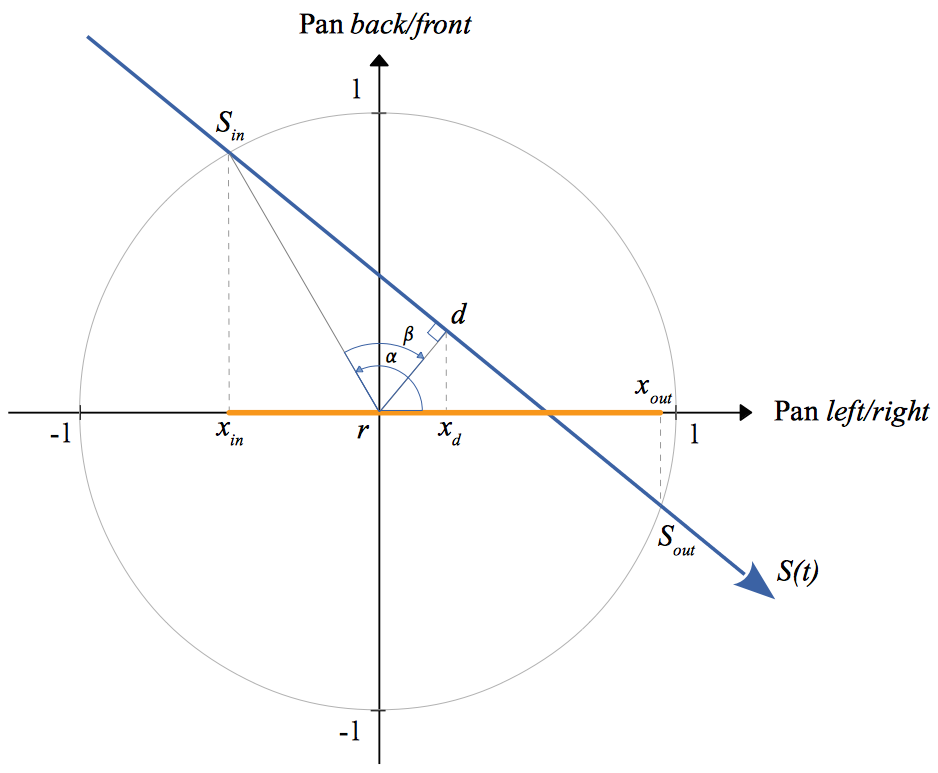
\includegraphics[scale=0.33]{img/4782}
\caption{Trajectoire de l'objet sonore $S(t)$ par rapport au r\'ecepteur $r$. }
\label{tra}
\end{center}
\end{figure}

\subsection*{Trajectoire de l'objet sonore}

La trajectoire est calcul\'ee \`a partir de quatre param\`etres qui vont conditionn\'e le panoramique. Ainsi, le point \'emergent $S_{in}$ est localis\'e  sur l'axe des ordonn\'ees par rapport \`a l'axe des abscisses -- d\'efinit par le param\`etre $x_{in}$ -- et indiqu\'e par le signe de $q$  ($+1$ ou $-1$) d\'eterminant respectivement le panoramique \textit{front/back} du point d'\'emergence. Dans le cas de la figure \ref{tra}, la valeur de  $q=+1$.%

\begin{enumerate}
\item Coordonn\'ees de $S_{in}$:\\  
Soit $\alpha = cos^{-1} \,x_{in}$;\\
$y_{in}=q\, sin \alpha$
\item Coordonn\'ees de $d$:\\ 
Soit $\beta = cos^{-1} \, d$;\\

$
   x_{d}=
\begin{dcases}
    d\, cos(\alpha + \beta)& \text{si } x_{in}>0\\
    d\, cos(\alpha - \beta)& \text{si } x_{in}<0
\end{dcases}
$

 Soit $\gamma =cos^{-1} \displaystyle \frac{x_d}{d}=\widehat{drx_d}$;\\
 $y_d=d\, q \,sin \gamma$
 \end{enumerate}
 
 \bigskip
 
 Pour d\'eterminer $S(t)$, il reste \`a \'evaluer $m$, c'est \`a dire le coefficient directeur (celui-ci d\'etermine le sens du panoramique, \`a savoir pour $m>0$ de la droite vers la gauche, et $m<0$ de la gauche vers la droite) et l'ordonn\'ee \`a l'origine $p$ (qui d\'etermine si la source passe \`a notre gauche pour $p>0$ ou \`a notre droite pour $p<0$ ) en fonction du panoramique de d\'epart $x_{in}$ (point d'emergence auditive) et de la distance $d$ de passage (au plus pr\`es) de la source au r\'ecepteur $r$.
 
 \begin{enumerate}[resume]
\item Calcul de la pente $m$ de $S(t)$:\\ 
$m=\displaystyle \frac{y_{in} - y_d}{x_{in} - x_d}$
\item Calcul de l'ordonn\'ee \`a l'origine $p$ de $S(t)$:\\ 
$p=y_{in} - m \, x_{in}$
 \end{enumerate}
 
 \bigskip
 
\noindent Enfin, il reste \`a localiser le point de fuite d\'efinit en $S_{out}$. 

 \begin{enumerate}[resume]
\item D\'eterminer $x_{out}$ afin de d\'efinir l'ambitus panoramique sur l'axe des abscisses:\\ 
Soit $x^2+y^2=1$ (selon le th\'eor\`eme de Pythagore),
la substitution de $y$ par $mx+p$ implique la r\'esolution d'une \'equation du second degr\'e de type: $ax^2+bx+c=0$,\\
Ainsi, pour:\\
\begin{description}
\item $a=m^2+1$
\item $b=2mp$
\item $c=p^2-1$
\end{description}
$
   x_{out}=
\begin{dcases}
    \frac{-b-\sqrt{\Delta}}{2a}& \text{si } x_{in}>0\\
    \frac{-b+\sqrt{\Delta}}{2a}& \text{si } x_{in}<0
\end{dcases}
\text{ avec } \Delta=b^2-4ac
$
\end{enumerate}

\subsection*{Evaluation de la distance}

La distance s'inscrit dans une perspective dynamique dans le champs audible en termes de filtre passe-bas (\textit{cutoff frequency} du LPF) combin\'e avec l'amplitude qui sera appliqu\'ee -- le cas \'ech\'eant -- au \textit{drylevel} de la reverb\'eration, en fonction de la localisation radial par rapport \`a $r$.%

\subsubsection*{Niveau sonore et Filtrage}

See appendice \fullref{dist}.
%Voir Annex 4 \nameref{Distance} p. \pageref{Distance}.

\subsubsection*{Elevation}

Dans le contexte pr\'esent, l'\'el\'evation consiste \`a `rectifier' la trajectoire par rapport \`a l'auditeur en conservant le niveau sonore d\'efinit par la distance de passage au plus pr\`es.%

\normalfont

\subsection*{Effet Doppler}

La fr\'equence per\c{c}u par l'auditeur (\myuline{r\'ecepteur immobile}) est d\'efinit par la formule,
$f_r= \displaystyle f_S  \frac{1}{\displaystyle 1- \frac{v_s \, cos \theta}{v}}$
avec $f$ pour la fr\'equence, $v$ pour la vitesse (du son sans indice), $r$ le r\'ecepteur et $S$ la source, $\theta$ est l'angle que fait la direction de la source avec le r\'ecepteur.

Au m\^eme titre concernant la relativit\'e du seuil de perception d\'ej\`a \'evoqu\'ee pour les points $S_{in}$ et $S_{out}$, le temps $tps$ que prendra la source en terme de vitesse pour parcourir l'ambitus panoramique sera relatif. 

Le rapport vitesse de la source par la vitesse du son dans l'atmosph\`ere sera par cons\'equent remplac\'e par l'inverse du temps relatif soit $tps^{-1}$, alors $f_r=f_S \displaystyle \frac{1}{1- \displaystyle \frac{cos \, \theta}{tps}}$ avec $\theta$ la coordonn\'ee angulaire de l'objet sonore \`a l'instant $t$, toujours par rapport \`a l'auditeur.

\newpage

\noindent \textbf{{\large Configuration spatiale}}
\hrulefill

  \bigskip
  
  \`A noter que dans le cadre de la performance \textit{in situ} (voir figures \ref{elg} et  \ref{pan}), chaque haut-parleur est dirig\'e vers l'ext\'erieur, en direction des murs et selon un angle estim\'e empiriquement afin d'\'eviter le son direct et de profiter de la premi\`ere reflexion comme substitut au signal direct. Cela n'est certes pas tr\`es orthodoxe mais s'avère efficace dans la configuration \textit{in situ} et selon le mat\'eriel \`a disposition -- \`a savoir 2 monitorings Yamaha HS80M plus 2 monitorings Yamaha HS50M (ces derniers sont plac\'es vers l'avant) et une carte son Motu ultralite mk3.
  
 \begin{figure}[H]
  \hspace{-1.2cm}
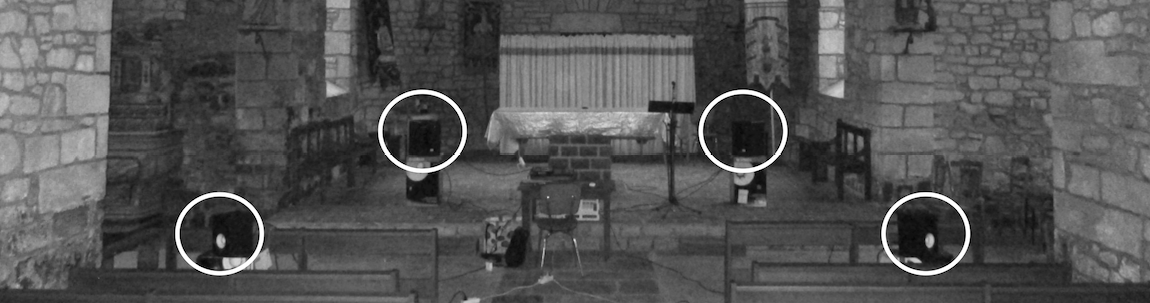
\includegraphics[scale=0.36]{img/5923}
\caption{\'Eglise de Lescou\"et-Gouarec -- Septembre 2015.}
\label{elg}
\end{figure}

\subsection*{Distribution des amplitudes dans l'espace quadriphonique}

\bigskip
\bigskip

\begin{center}
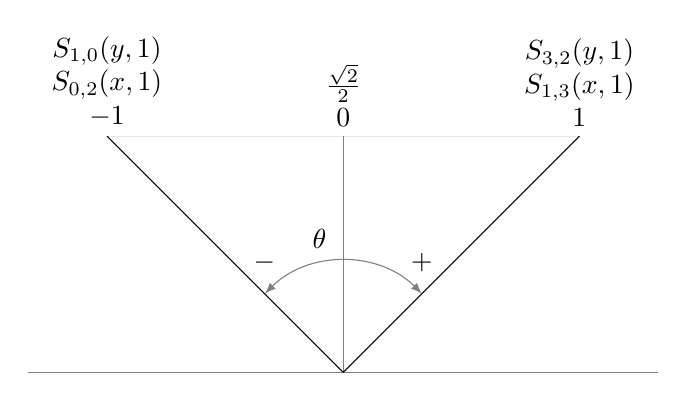
\begin{tikzpicture}[every text node part/.style={align=center}]
\draw[gray] (0,0) -- (8,0);
\draw[gray!20] (1,3) -- (7,3);
\draw[gray] (4,0) -- (4,3) node[above,black]{$\frac{\sqrt{2}}{2}$ \\ $0$}
;
\draw (4,0) -- (1,3) node[above,]{$S_{1,0} (y,1)$ \\ $S_{0,2} (x,1)$ \\ $-1$};
\draw (4,0) -- (7,3) node[above]{$S_{3,2} (y,1)$ \\ $S_{1,3} (x,1)$ \\ $1$};
\draw[gray, <->,>=latex] (5, 1) arc (45: 135: 1.41cm);
\node at (3.7,1.7) {$\theta$};
\node at (3,1.4) {$-$};
\node at (5,1.4) {$+$};
\end{tikzpicture}
\end{center}

\bigskip

Soit $\theta$ l'angle en coordonn\'ee polaire du point $([-1,1],1)$; le retranchement par $\frac{\pi}{2}$ permet de d\'efinir un intervalle  $\theta \in [ - \frac{\pi}{4}, \frac{\pi}{4}]$.

\smallskip

\noindent Ainsi, la panoramisation \`a puissance constante est d\'efinit par \citep[ p. 134]{cr}:
\smallskip

$S_{1,0/0,2} = \frac{\sqrt{2}}{2} \: [ \: cos \: \theta + sin \: \theta \: ]$

$S_{3,2/1,3} = \frac{\sqrt{2}}{2} \: [ \: cos \: \theta - sin \: \theta \: ]$

\smallskip

\noindent Telle que:

$S_0=S_{0,2} \times S_{1,0}$

$S_1=S_{1,3} \times S_{1,0}$

$S_2=S_{0,2} \times S_{3,2}$

$S_3=S_{1,3} \times S_{3,2}$

\smallskip

\noindent De sorte \`a confirmer l'\'egalité suivante:

\smallskip

$\displaystyle \sum_{i=1}^{n} (S_{i-1})^2 =1$ avec $n=4$, soit 4 haut-parleurs. 

 \begin{figure}[H]
\begin{center}
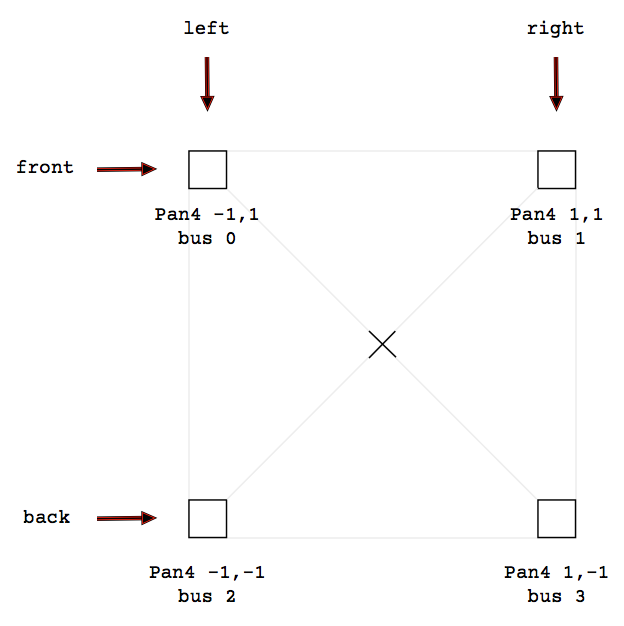
\includegraphics[scale=0.5]{img/6643}
\caption{Panoramique quadriphonique de \textit{Triptyque}, tel qu'il est interpr\'et\'e avec l'\textit{UGen} \texttt{Pan4} avec les num\'eros de bus respectifs. }
\label{pan}
\end{center}
\end{figure}

\newpage

\noindent \textbf{{\large Tree-like format of \textit{Triptyque}}}
\hrulefill

 \begin{figure}[H]
\begin{center}
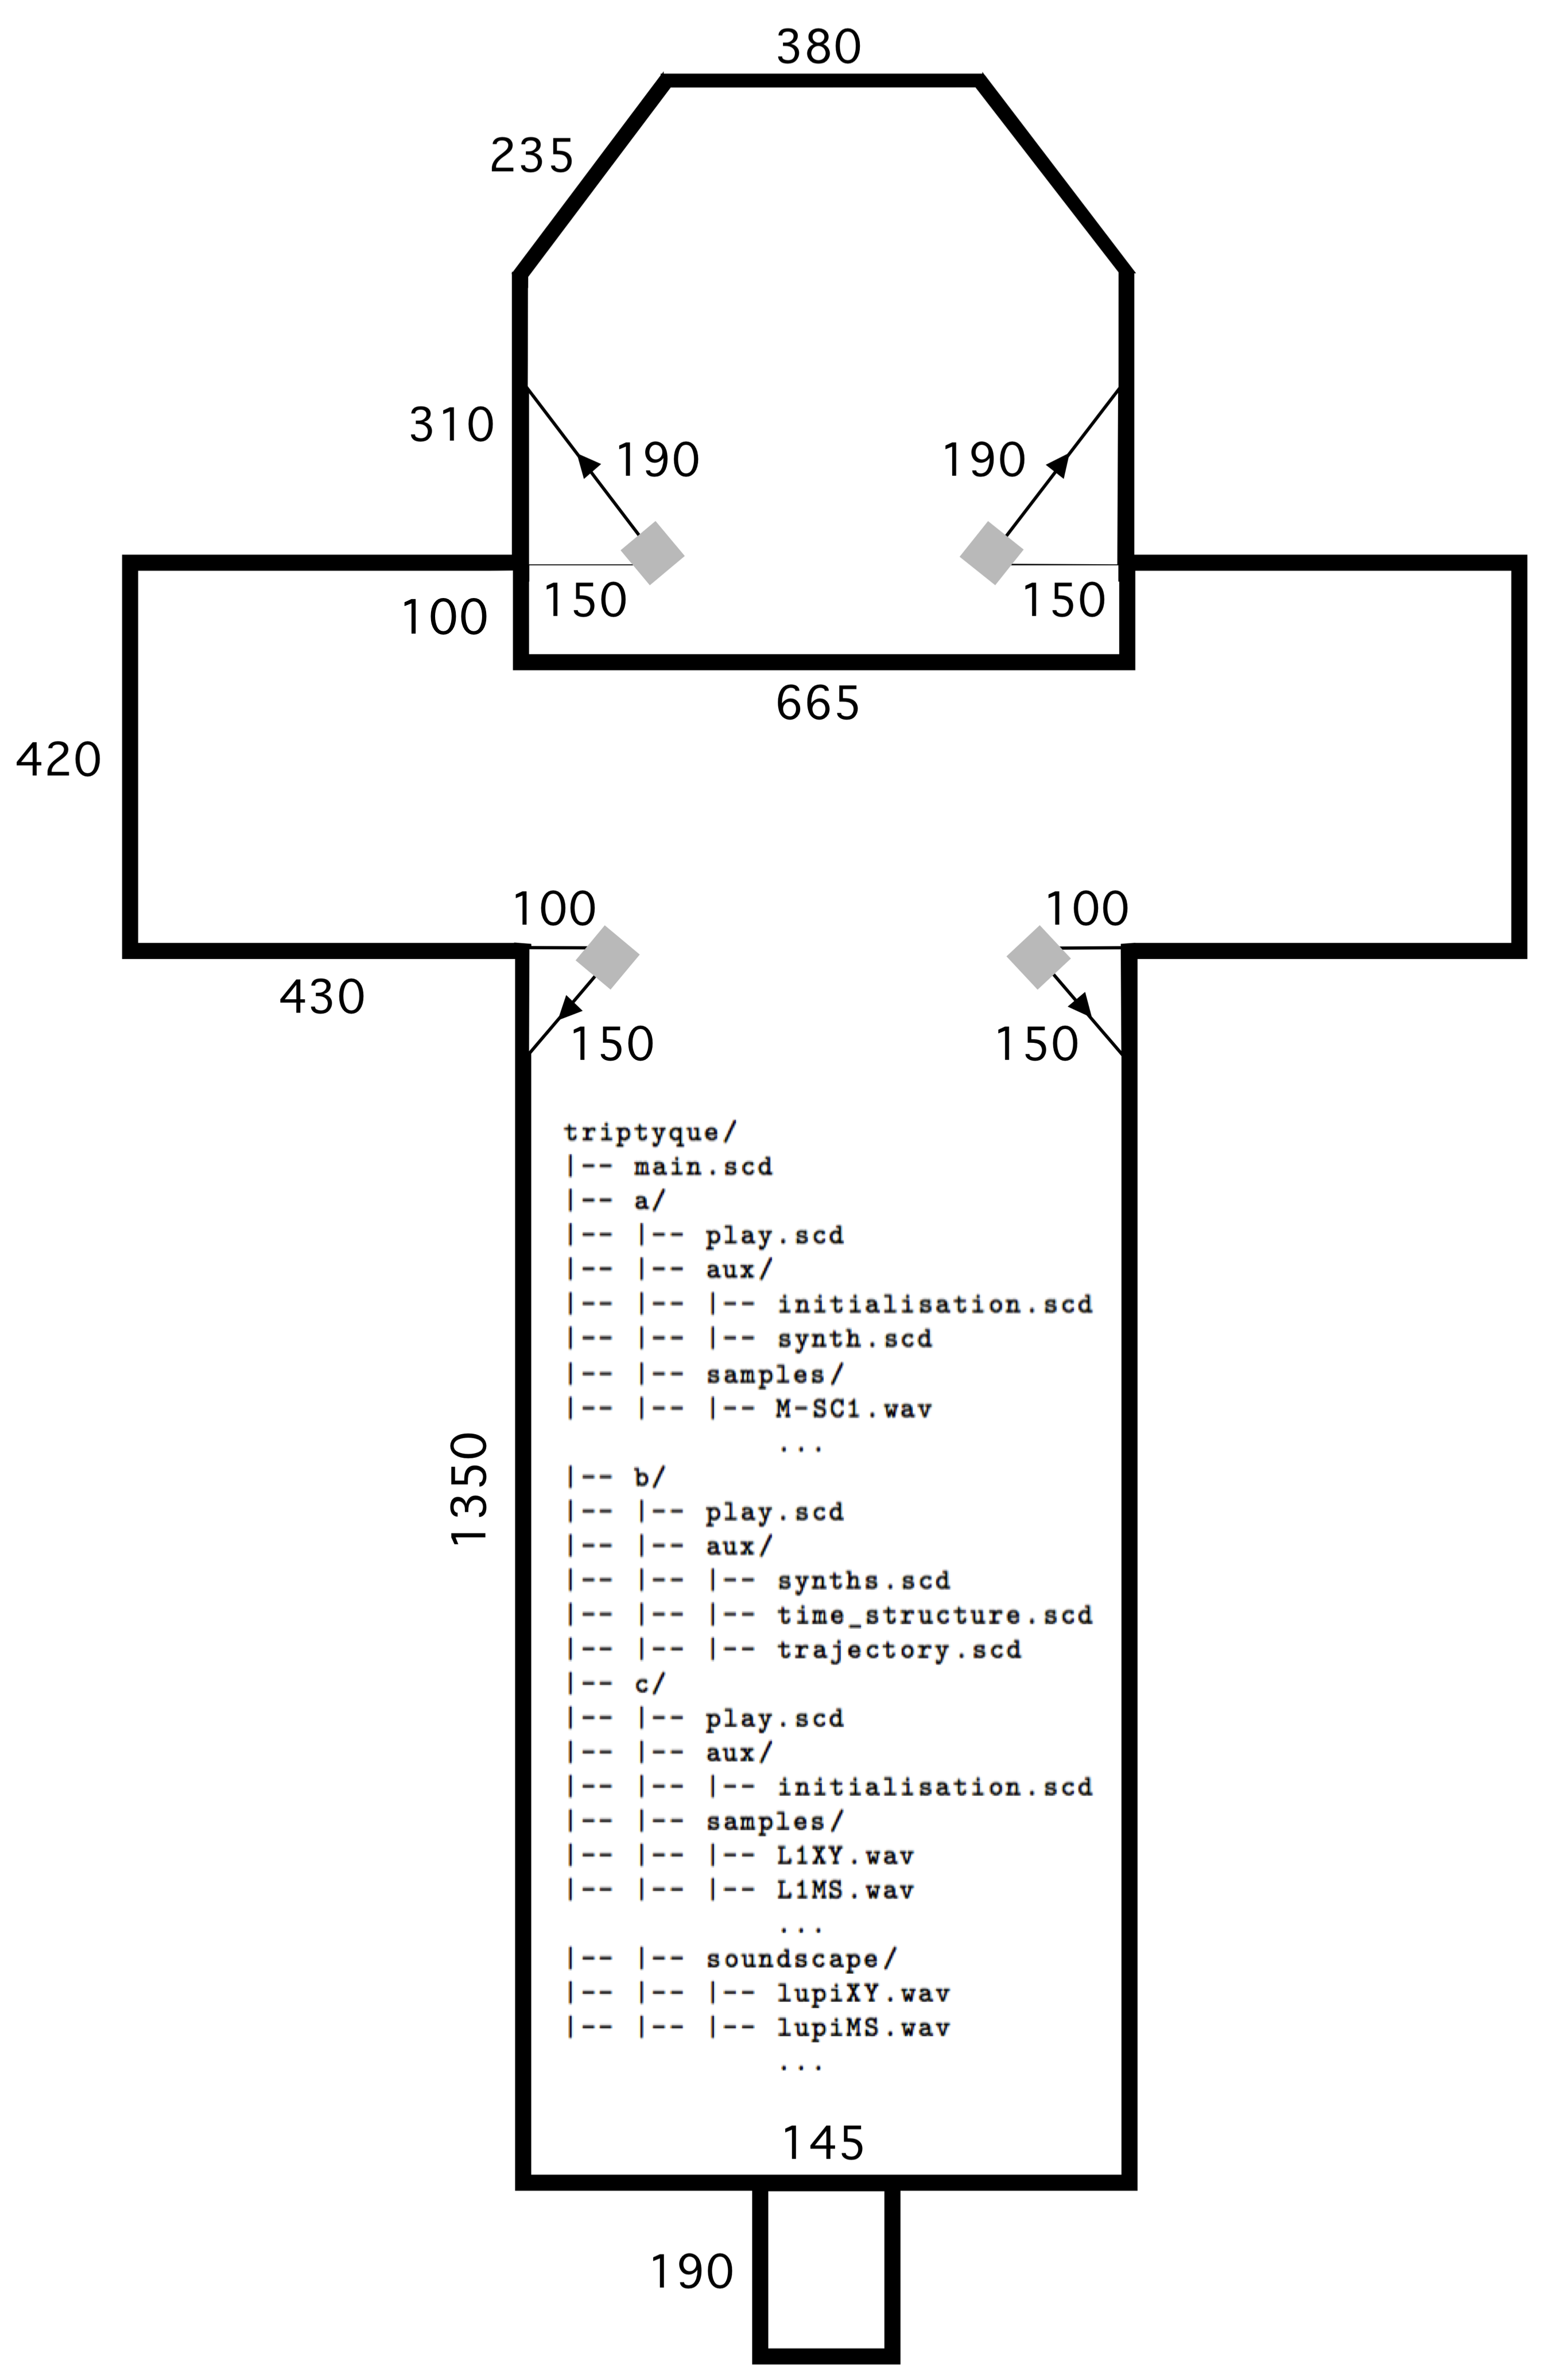
\includegraphics[width=0.9\textwidth]{img/4361.png}
\end{center}
\end{figure}

%Le mode d'enregistrement décrit en figure \ref{h2n} concerne les samples des répertoires {/triptyque/c/samples/} et {/triptyque/c/soundscape/}.